\documentclass[journal]{IEEEtran}
\IEEEoverridecommandlockouts
\usepackage{etoolbox}
\makeatletter
\patchcmd{\abstract}{---}{-}{}{}
\patchcmd{\IEEEkeywords}{---}{-}{}{}
\makeatother
\usepackage{cite}
\usepackage{amsmath,amssymb,amsfonts}
\usepackage{algorithmic}
\usepackage{graphicx}
\usepackage{textcomp}
\usepackage{xcolor}
\usepackage{colortbl}
\usepackage{booktabs}
\usepackage{multirow}
\usepackage{balance}
\usepackage[hidelinks]{hyperref}
\usepackage{microtype}
\usepackage{tikz}
\usetikzlibrary{arrows, positioning, calc}

\def\BibTeX{{\rm B\kern-.05em{\sc i\kern-.025em b}\kern-.08em
    T\kern-.1667em\lower.7ex\hbox{E}\kern-.125emX}}

\begin{document}

\title{Multilingual Spam Email Detection for English and Bangla Messages using QLoRA-Fine-Tuned Large Language Models with Explainable AI Validation}

\author{Najmush Shakib and Munim Halder \\
\textit{Department of Computer Science and Engineering} \\
\textit{Bangladesh University of Business and Technology (BUBT)} \\
Dhaka, Bangladesh \\
nstasin81@gmail.com, munimhalder666@gmail.com
}

\maketitle

\begin{abstract}
Global messaging platforms are experiencing a surge
in spam, phishing, and smishing attacks, which impose significant
The financial and security expenses for users. Although current spam
detection algorithms perform exceptionally well for resource-
rich languages like English, low-resource languages such as
Bangla (with over 230 million speakers) lack robust support
From both commercial and academic filters; in order to fill this gap, this
paper introduces a unified multilingual framework that classifies
English and Bangla spam occur at the same time. This method
eliminates the need for language-specific feature engineering
or by using separate processing pipelines. We used Quantized Low-
Rank Adaptation (QLoRA) to fine-tune five compact, pre-trained
Large Language Models (such as Phi-3.5 Mini to SmolLM2-
360M) on a combined dataset of standard SMS spam and
Phishing messages that are in native Bangla. Our preprocessing pipeline
incorporates Unicode normalization, URL token substitution, and
a group-aware splitting strategy designed to prevent data leakage
During the training process, we used the Synthetic Minority Over-sampling method.
Technique (SMOTE) exclusively within the training feature space
To balance the classes without compromising the validation sets, the model should. Performance was evaluated using standard metrics across both languages, and McNemar’s test was used to verify the statistical
The importance of the results. Moreover, an Explainable AI (XAI)
module based on cross-layer attention aggregation was included
to ensure that predictions rely on semantically relevant features
not just superficial artifacts; the experimental results show
that fine-tuning compact LLMs via QLoRA is a highly parameter-
An efficient method, reaching a peak accuracy of 98.24 percent on the bilingual task and outperforming traditional machine learning
baselines.
\end{abstract}

\begin{IEEEkeywords}
Index Terms-Spam Detection, Bangla NLP, QLoRA, Large
Language Models, Parameter-Efficient Fine-Tuning, PEFT, Ex-
plainable AI, Multilingual Classification, Phishing Detection,
Smishing
\end{IEEEkeywords}

\section{Introduction}

\subsection{Background and Motivation}

\IEEEPARstart{U}{nwanted} electronic messages, commonly known as
spam, pose a serious security and economic challenge in modern digital communication. Beyond being a nuisance, spam serves as a primary vector for phishing attacks, malware distribution, and financial fraud, leading to billions of dollars in annual losses~\cite{ref1}. The use of mobile messaging apps, like SMS and WhatsApp has made things more dangerous. Bad people often try ways to get around security. They change how they speak and mix languages. This makes old ways of stopping messages not work anymore.~\cite{ref5},~\cite{ref6}.

People have made some improvements in the way computers understand language, which is called natural language processing and in machine learning. These improvements have helped create tools that can figure out what things mean. These tools use statistics and other methods like looking at words in a way using something called recurrent neural networks and a new kind of model called transformer-based pre-trained language models. They are really good, at understanding natural language processing and machine learning. Natural language processing and machine learning are used to make these tools better.~\cite{ref4},~\cite{ref7},~\cite{ref9}. These developments have pushed detection accuracies on English language benchmarks to saturation, with several systems achieving over 98\% accuracy on established datasets like the SMS Spam Collection~\cite{ref1} and Enron Email~\cite{ref9}. Although these successes have been achieved, cross-lingual generalization is still mostly an unsolved problem.

The fact that low-resource languages such as Bangla have this limitation is especially clear, since although Bangla is spoken by a huge number of people around the world, it still has very little computational linguistic support. In Bangladesh digital communication generally combines the native Bangla script, romanized phonetics, English words borrowed into the language, and mixed code-switching. At the same time, the quick growth of local mobile financial services (MFS), for example bKash and Nagad, has led to the emergence of phishing attacks that are tailored to the local context and take advantage of users' trust in these services. Even advanced Bangla text classifiers, which perform well on standard academic benchmarks~\cite{ref7}, they often have difficulty dealing with these new and localized kinds of threats.

\subsection{Problem Statement}

Current research approaches generally bifurcate into two
isolated streams: resource-rich English frameworks with ad-
vanced architectural capabilities, and specialized monolingual
Models that have been designed specifically for localized dialects. Many
Bangla-focused systems rely on deep learning models that
require extensive annotated datasets, significant computational
resources, or custom feature extraction mechanisms that struggle to generalize against novel attack vectors~\cite{ref7},~\cite{ref10}. So far, there has been no published system which incorporates English and Bangla spam detection into one unified end-to-end model without having to use language-specific preprocessing pipelines or special Bangla tokenizers.

The fact that there is such architectural isolation leads to a great deal of operational overhead. In live production situations—for example, in telecom networks or in financial institutions which operate in bilingual settings—running separate pipelines for each language results in unnecessary overhead, higher maintenance costs, and increased complexity. Because of this, there is a strong operational need to develop a single model which is able to process raw text in both languages and at the same time provide explainable classifications.

\subsection{Proposed Solution and Contributions}

In order to deal with these challenges, we offer a single, unified framework for detecting spam in multiple languages. Our method involves fine-tuning publicly available, compact Large Language Models (LLMs) using Quantized Low-Rank Adaptation (QLoRA)~\cite{ref11}. By updating less than 1\% of the model weights, QLoRA allows billion-parameter models to be adapted for specific classification tasks. This greatly lowers the memory and computational demands so that LLMs can be fine-tuned using a standard consumer GPU or in a cloud-based environment. The level of efficiency is especially advantageous for low-resource languages, since the costs associated with full pre-training or standard fine-tuning are frequently prohibitive.

The primary contributions of this paper are:

\textbf{1) Unified Bilingual Classification Framework:} We have designed and evaluated a single pipeline based on an LLM which is able to detect spam in both English and Bangla, without needing language-specific branching or the use of custom feature extraction.

\textbf{2) Template-Aware, Leakage-Free Dataset Construction:} We present a method for splitting the data in the Bangla dataset which divides the records according to their underlying message template IDs. This approach stops nearly identical messages from occurring in both the training and test sets, thus overcoming a significant yet often neglected data leakage problem in Bangla NLP research.

\textbf{3) Standardized Multi-Model Comparative Study:} We use the same hyperparameters and experimental conditions to fine-tune and evaluate five different LLMs (ranging in size from 360 million to 3.8 billion parameters). This enables a rigorous baseline comparison of the performance of smaller models on the task of bilingual classification.

\textbf{4) Explainability via Attention Weight Visualization:} We incorporate a cross-layer attention aggregation mechanism into the classification pipeline so that token importance scores can be obtained, enabling researchers and practitioners to check that the model's predictions are based on semantically meaningful content rather than on spurious artifacts.

\textbf{5) Statistical Significance Testing:} To verify the performance differences among the top-performing models we use McNemar's non-parametric test, in order that our comparative results may be considered statistically robust rather than merely the result of sampling variance.



\section{Related Work}

The classification of spam, phishing, and smishing messages has been looked at in great detail. For example, there is the SMS Spam Collection~\cite{ref1} used traditional algorithms such as Support Vector Machines (SVM) and Naïve Bayes~\cite{ref1},~\cite{ref5}, achieving high accuracy but struggling with deep semantic understanding. Feature-based solutions for URL phishing detection~\cite{ref2},~\cite{ref8} demonstrated high efficacy but remained vulnerable to evasion tactics like non-HTML obfuscation.

Subsequent research shifted toward neural sequence models. Dutta~\cite{ref3} applied RNN-LSTMs for zero-day phishing URL detection, while SpamDL~\cite{ref9} combined GloVe vectors with Bi-LSTMs for email classification. For mobile messaging, hybrid architectures like SmishGuard~\cite{ref6} and multi-signal NLP frameworks~\cite{ref10} significantly improved detection reliability. However, these systems were explicitly designed for English corpora, lacking mechanisms for cross-lingual transfer.

In the context of Bangla text classification, transformer-based multilingual architectures have shown promise. Alam et al.~\cite{ref4} explored mBERT and XLM-RoBERTa, noting that subword tokenization often dilutes semantic information for resource-limited languages. Talukder et al.~\cite{ref7} achieved state-of-the-art results on Bangla SMS using BiLSTM and 1D-CNN architectures, but their system was inherently monolingual.

\subsection{Synthesis and Research Gap}

There is a clear linguistic divide in the literature. Although there are highly accurate and advanced models available for detecting English spam, research involving Bangla is limited in terms of the scope, variety of datasets, and the modernisation of its architecture. As far as we know, no previous study has managed to fine-tune a single, unified model architecture so as to deal with both languages at the same time.

There are common deficiencies in the approaches used by
previous researchers in the field which include lack of attention to
data leakage in template-based datasets, use of monolingual datasets
only, and lack of methods for explainability of the model to enable its
The main features of the one examined are concerned with use in cybersecurity practice,
studies are given in Table~\ref{tab:comparative}.

\begin{table}[htbp]
\caption{Comparative Summary of Methods}
\label{tab:comparative}
\centering
\begin{tabular}{lllc}
\toprule
\textbf{Ref.} & \textbf{Dataset} & \textbf{Architecture} & \textbf{Acc.} \\
\midrule
\cite{ref1} & SMS Spam Collection (5,574) & SVM, NB & 97.64\% \\
\cite{ref2} & 6,000 URLs & XGBoost & 99.17\% \\
\cite{ref3} & PhishTank ($\sim$13k URLs) & RNN-LSTM & 97.40\% \\
\cite{ref4} & 6 Bangla datasets & mBERT & 93.80\% \\
\cite{ref5} & SMS Spam v1 (5,169) & NB + Dict. & 96.20\% \\
\cite{ref6} & SMS Phishing (7,261) & XGBoost & 98.47\% \\
\cite{ref7} & 11,599 Bangla SMS & BiLSTM & 99.00\% \\
\cite{ref8} & URL phishing DB & SVM, LR & 91.40\% \\
\cite{ref9} & Enron + SpamAssassin & Bi-LSTM & $\sim$98\% \\
\cite{ref10} & 84,000 global SMS & Multi-NLP & 97.89\% \\
\textbf{Ours} & \textbf{Eng + Bangla (7,924)} & \textbf{QLoRA LLM} & \textbf{98.24\%} \\
\bottomrule
\end{tabular}
\end{table}

We deal with these gaps by (a) preparing a bilingual training corpus, (b) introducing a leakage-free, group-aware data split, (c) making use of the multilingual capabilities of pre-trained LLMs through parameter-efficient fine-tuning, and (d) including XAI techniques in order to achieve model interpretability.



\section{Methodology}

The following section describes the experimental setup and sets out the learning task. The methodology is made up of five main stages: (A) problem formulation, (B) dataset preparation, (C) preprocessing, (D) data splitting and leakage prevention, and (E) architecture design and training.

\subsection{Problem Formulation}

The task of multilingual spam detection is modeled as a supervised binary sequence classification problem. Let $\mathcal{D} = \{(x_i, y_i)\}_{i=1}^{N}$ denote a dataset consisting of $N$ text messages, where each message $x_i$ is a sequence of tokens from a vocabulary $\mathcal{V}$ that spans multiple languages (in this context, English and Bangla). The corresponding label $y_i \in \{0, 1\}$ denotes whether the message is legitimate (ham, $y_i = 0$) or malicious (spam/phishing, $y_i = 1$). 

The objective is to learn a mapping function $f_\theta: \mathcal{X} \rightarrow \mathcal{Y}$, parameterized by $\theta$, such that the predicted label $\hat{y}_i = f_\theta(x_i)$ minimizes the standard cross-entropy loss over the dataset:
\begin{equation}
\mathcal{L}(\theta) = -\frac{1}{N} \sum_{i=1}^{N} \left[ y_i \log f_\theta(x_i) + (1 - y_i) \log (1 - f_\theta(x_i)) \right]
\end{equation}
Unlike traditional approaches that require language-identification branching, $f_\theta$ must inherently capture cross-lingual semantic representations within a unified embedding space. In this work, $f_\theta$ represents a pre-trained causal language model adapted for classification, and we seek to find optimal parameters $\theta^*$ using a low-rank approximation strategy to minimize computational overhead.

\begin{figure}[htbp]
\centering
\resizebox{\columnwidth}{!}{
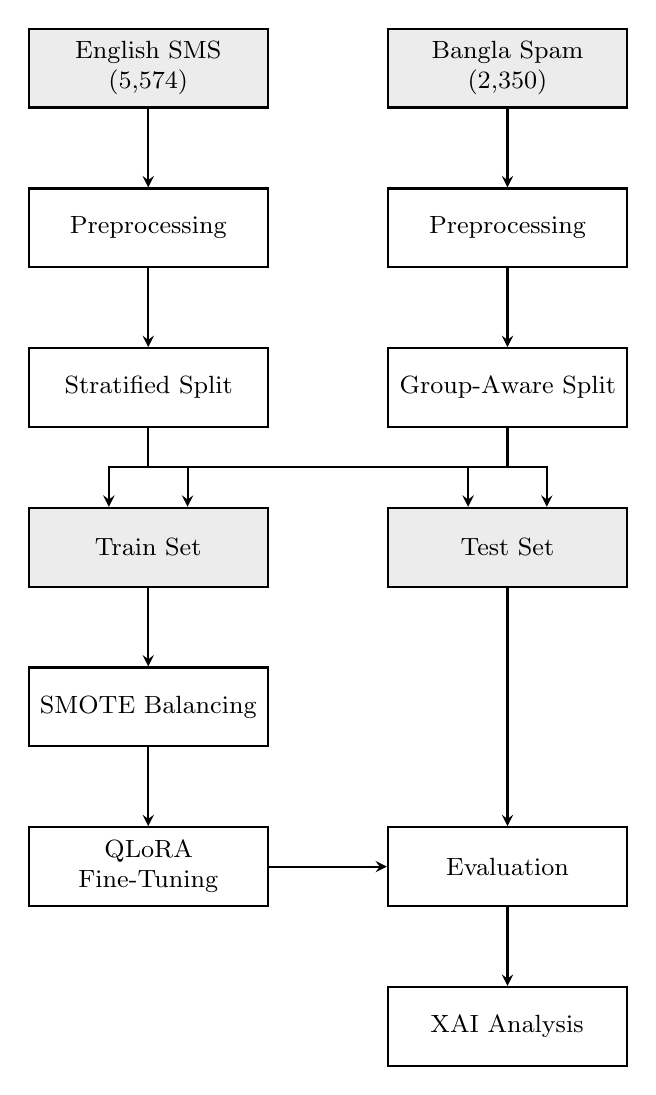
\begin{tikzpicture}[
    node distance=1cm and 1.5cm,
    box/.style={rectangle, draw=black, thick, fill=white, minimum width=3cm, minimum height=1cm, text centered, text width=2.8cm, font=\small},
    data/.style={rectangle, draw=black, thick, fill=gray!15, minimum width=3cm, minimum height=1cm, text centered, text width=2.8cm, font=\small},
    arrow/.style={thick, ->, >=stealth, draw=black}
]
\node (eng) [data] {English SMS\\(5,574)};
\node (ben) [data, right=1.5cm of eng] {Bangla Spam\\(2,350)};
\node (prep_eng) [box, below=of eng] {Preprocessing};
\node (prep_ben) [box, below=of ben] {Preprocessing};
\node (split_eng) [box, below=of prep_eng] {Stratified Split};
\node (split_ben) [box, below=of prep_ben] {Group-Aware Split};
\node (train) [data, below=1cm of split_eng] {Train Set};
\node (test) [data, below=1cm of split_ben] {Test Set};
\node (smote) [box, below=of train] {SMOTE Balancing};
\node (qlora) [box, below=of smote] {QLoRA Fine-Tuning};
\node (eval) [box] at (test |- qlora) {Evaluation};
\node (xai) [box, below=of eval] {XAI Analysis};

\draw [arrow] (eng) -- (prep_eng);
\draw [arrow] (ben) -- (prep_ben);
\draw [arrow] (prep_eng) -- (split_eng);
\draw [arrow] (prep_ben) -- (split_ben);
\draw [arrow] (split_eng.south) -- ++(0,-0.5) -| ([xshift=-0.5cm]train.north);
\draw [arrow] (split_eng.south) -- ++(0,-0.5) -| ([xshift=-0.5cm]test.north);
\draw [arrow] (split_ben.south) -- ++(0,-0.5) -| ([xshift=0.5cm]train.north);
\draw [arrow] (split_ben.south) -- ++(0,-0.5) -| ([xshift=0.5cm]test.north);
\draw [arrow] (train) -- (smote);
\draw [arrow] (smote) -- (qlora);
\draw [arrow] (test) -- (eval);
\draw [arrow] (qlora) -- (eval);
\draw [arrow] (eval) -- (xai);
\end{tikzpicture}
}
\caption{End-to-End Methodology Framework}
\label{fig:methodology}
\end{figure}

\subsection{Dataset Construction and Description}

The study uses two distinct corpora that are combined into a single
bilingual training and evaluation dataset.

\textit{1) English Corpus - SMS Spam Collection:} The part of the dataset in English was obtained from the SMS Spam Collection dataset introduced by Almeida et al.~\cite{ref1}. This data set contains 5,572 SMS messages in
The messages are hand-labeled as either "ham" or "spam". The dataset shows a considerable imbalance between the classes: about 86.6\% of the messages are genuine (ham) and 13.4\% are spam; this
distribution closely mirrors real-world communication flows, necessitating
There are some effective techniques for balancing classes. The messages in this data set are stored as
plain UTF-8 strings.

\textit{2) Bangla Corpus - Phishing and Promotional Spam Dataset:} The
Bangla dataset comprises a native language corpus of phishing and
promotional spam gathered from Bangladesh digital communication
The dataset contains messages representing various
categories of malware, including MFS fraud, phishing messages under the
guise of bKash and Nagad, lottery, prize and promotional spam, as well
as transactional and conversational messages, which constitute the ham
Each entry in the Bangla dataset has a template\_id field which shows the template it is based on. This attribute allows for a group-aware approach.
splitting technique discussed in Section III.C. The labeling scheme for
the binary classification task is identical to the one for the English
Dataset 0 is ham while dataset 1 is spam.

The summary of both datasets prior to preprocessing is shown in Table
II.

\begin{table}[htbp]
\caption{Dataset Composition Before Preprocessing}
\label{tab:dataset_raw}
\centering
\begin{tabular}{lll}
\toprule
\textbf{Attribute} & \textbf{English (SMS Spam)} & \textbf{Bangla (Phishing/Spam)} \\
\midrule
Total Records & 5,572 & 3,114 \\
Ham (Label = 0) & $\sim$4,825 & 1,443 \\
Spam (Label = 1) & $\sim$747 & 1,671 \\
Language & English & Bangla (code-mixed) \\
Source & Public repo \cite{ref1} & Native corpus \\
Template Metadata & None & template\_id per record \\
\bottomrule
\end{tabular}
\end{table}

\subsection{Preprocessing Pipeline}

The main aim of the preprocessing pipeline was to guarantee textual consistency in both languages. Stemming and the removal of stop words were deliberately left out since these operations usually remove context that is semantically important in malicious emails and interfere with the parsing logic of multilingual tokenizers working with the Bangla script.

\textit{1) Garbage Character Removal:} Raw text fields across both corpora were initially sanitized. Newline (\textbackslash n), carriage return (\textbackslash r), and tab (\textbackslash t) characters were replaced with single spaces, and leading or trailing whitespace was stripped to establish a normalized text baseline.

\textit{2) Unicode Normalization:} The integration of distinct writing systems frequently introduces encoding inconsistencies. To resolve this, all text strings were processed using NFKC normalization via Python's \texttt{unicodedata} library. This process breaks compatibility characters down into their canonical forms and recomposes them, guaranteeing a uniform encoding standard before the text reaches the tokenizer.

\textit{3) URL and Numeric Token Replacement:} Because embedded URLs are a primary vector for phishing campaigns, regular expressions targeting standard \texttt{http}/\texttt{https} schemes and \texttt{www}-prefixed hostnames were used to substitute malicious links with a generic \texttt{URL} placeholder. A parallel substitution replaced standalone digits with a \texttt{NUMBER} token. This approach preserves the semantic indicator of a link or numeric sequence without exhausting the tokenizer's vocabulary limit on unique, high-entropy character strings.

\textit{4) Missing Value and Duplicate Removal:} All records which
contained null or blank fields in either the text or label columns
Were left out of both datasets. The duplicates were detected
based on an exact match of text string and only one instance
Each message was retained. The number of records before and
The details of each cleaning step are given in Table~\ref{tab:dataset_prep}
below.

\begin{table}[htbp]
\caption{Record Counts After Each Preprocessing Stage}
\label{tab:dataset_prep}
\centering
\begin{tabular}{lcc}
\toprule
\textbf{Stage} & \textbf{English Records} & \textbf{Bangla Records} \\
\midrule
Raw & 5,572 & 3,114 \\
After Null Removal & 5,500 & 2,280 \\
After Deduplication & 5,170 & 2,205 \\
Final & 5,170 & 2,205 \\
\bottomrule
\end{tabular}
\end{table}

\textit{5) Label Encoding Verification:} An audit of the label encodings for both datasets in a programmatic way confirmed strict binary compliance, thus verifying that the label vectors contained only 0 (ham) and 1 (spam) values.

\subsection{Data Partitioning and Leakage Prevention}

Since the Bangla dataset contains structural templates, standard random partitioning was not adequate for the combined corpus; randomly splitting these records carries a great risk of data leakage, because the models are likely to overfit to the syntactic structure of particular templates rather than learn the underlying semantic threat indicators.

\textit{1) Bangla: Group-Aware Splitting via GroupShuffleSplit:} To mitigate this risk, the Bangla corpus was partitioned using scikit-learn's \texttt{GroupShuffleSplit}, utilizing the \texttt{template\_id} as the grouping variable. This guarantees that all instances of a specific template are routed exclusively to either the training or test set. Following a 20\% test allocation, post-split verification confirmed zero template intersection between the partitions.

\textit{2) English: Stratified Random Splitting:} Since the English corpus
does not contain template metadata, stratified random splitting with 20\%
test size and the same seed was applied to the corpus. Stratification
according to the label column ensures that the spam-to-ham class distribution in the training subset mirrors the overall English corpus.

\textit{3) Combination and Shuffle:} The English and Bangla training data
splits were joined together and randomly shuffled (random\_state=42) to
create one bilingual training dataset. The same process was applied to
the test data splits. The shuffle operation ensures that no model can
exploit any positional information linked to the order in
which the language-specific data splits were created. The dataset was
finally converted into Hugging Face Datasets for use with the Trainer
API in the later stages.

\textit{4) Leakage Verification:} The following are the three tests done
independently to verify the absence of any kind of leakage during the
partitioning process:

(a) Exact match intersection of the train and test text strings.

(b) Template intersection of the set of Bangla training and test
templates.

(c) TF-IDF vectorization in the SMOTE phase trained only on the
training partition.

All three of these verification steps independently confirmed exactly zero data leakage between the final training and testing partitions, ensuring the integrity of the evaluation metrics.

\subsection{Class Imbalance Handling via SMOTE}

The merged training dataset retains the inherent class
imbalance of the source corpora, with legitimate messages
outnumbering the spam examples by a large margin. When training a classifiercation model directly on this imbalanced distribution induces
a majority-class bias, yielding artificially high overall accuracy
while severely degrading recall on the minority spam class—the
A key measure in threat detection.

In order to counteract this imbalance, SMOTE was used only with the training subset.
SMOTE synthesizes minority class instances through interpolation in the
The feature space of the real minority instances and their k nearest neighbours.
To prevent test-set contamination during LLM fine-tuning, SMOTE had to be run in the TF-IDF feature space using a vectorizer
trained on the training data set alone using a vocabulary of 5,000
features; the resampled indices were then used to adjust the
The distribution of the training data set was considered, and the test data set was vectorized.
using the fitted but not the refitted vectorizer from the training data
set to reflect an actual inference scenario. Table~\ref{tab:smote} provides a summary
of the class distribution prior to and after running SMOTE.

\begin{table}[htbp]
\caption{Training Set Class Distribution Before and After SMOTE}
\label{tab:smote}
\centering
\begin{tabular}{lcc}
\toprule
\textbf{Class} & \textbf{Before SMOTE} & \textbf{After SMOTE} \\
\midrule
Ham (0) & 4,216 & 4,216 \\
Spam (1) & 1,684 & 4,216 \\
\textbf{Total} & \textbf{5,900} & \textbf{8,432} \\
\bottomrule
\end{tabular}
\end{table}

\subsection{Model Architectures and Selection Rationale}

Five distinct pre-trained Large Language Models (LLMs) were selected as base architectures. To ensure efficient token processing in Bangla, selection was restricted to models pre-trained on diverse multilingual corpora. Table~\ref{tab:models} outlines the selected models, all of which are publicly hosted on the Hugging Face Hub.

\begin{table}[htbp]
\caption{Selected Pretrained LLMs}
\label{tab:models}
\centering
\begin{tabular}{llc}
\toprule
\textbf{Model Name} & \textbf{Hugging Face ID} & \textbf{Parameters} \\
\midrule
Phi-3.5 Mini & microsoft/Phi-3.5-mini-instruct & $\sim$3.8B \\
Qwen2.5-1.5B & Qwen/Qwen2.5-1.5B-Instruct & $\sim$1.5B \\
TinyLlama-1.1B & TinyLlama/TinyLlama-1.1B-Chat-v1.0 & $\sim$1.1B \\
StableLM-2-1.6B & stabilityai/stablelm-2-1\_6b-chat & $\sim$1.6B \\
SmolLM2-360M & HuggingFaceTB/SmolLM2-360M-Instruct & $\sim$360M \\
\bottomrule
\end{tabular}
\end{table}

Model selection was guided by specific operational con-
The candidates were limited to parametric architectures.
eter sizes viable for fine-tuning on a single consumer-grade
With regard to the GPU, priority was given to the instruction-tuned variants, as
they generally provide superior zero-shot initialization for
Compared to raw foundational models, classification tasks are considered.
Finally, the selection intentionally spans a broad parameter
continuum, from 360 million to 3.8 billion, to empirically
evaluate the scaling relationship between computational effi-
ciency and classification accuracy.

\subsection{QLoRA Fine-Tuning Configuration}

Binary sequence classification fine-tuning was executed using Quantized Low-Rank Adaptation (QLoRA) \cite{ref11}. QLoRA integrates 4-bit weight quantization with low-rank adapters, facilitating the parameter-efficient adaptation of large-scale models within constrained memory footprints. The
particular quantization parameters used included Normal Float 4-bit
(nf4) quantization with double quantization set to True and fp16 for
activation tensors computations.

Adapter layers based on LoRA technology were embedded into the attention
projection matrices for each model. The target modules were selected
according to the naming convention of each model:
\begin{itemize}
    \item \textbf{Phi-3.5 Mini:} qkv\_proj, o\_proj, gate\_up\_proj, down\_proj
    \item \textbf{Qwen2.5 and StableLM-2:} q\_proj, k\_proj, v\_proj, o\_proj, gate\_proj, up\_proj, down\_proj
    \item \textbf{TinyLlama and SmolLM2:} q\_proj, k\_proj, v\_proj, o\_proj
\end{itemize}

The LoRA rank value was equal to r=16, the scale factor was set to
alpha=32, while the dropout probability was chosen to be equal to 0.05
resulting in less than 1\% of total model parameters being trainable.

\begin{table}[htbp]
\caption{QLoRA Hyperparameter Configuration}
\label{tab:qlora}
\centering
\begin{tabular}{ll}
\toprule
\textbf{Hyperparameter} & \textbf{Value} \\
\midrule
Quantization & 4-bit NF4 w/ double quant \\
Compute dtype & float16 \\
LoRA rank (r) & 16 \\
LoRA alpha & 32 \\
LoRA dropout & 0.05 \\
Target modules & Architecture-specific \\
Trainable params & $<$ 1\% of total \\
Task type & SEQ\_CLS \\
\bottomrule
\end{tabular}
\end{table}

\subsection{Training Protocol and Hyperparameters}

Models were trained via the Hugging Face Trainer API with an effective batch size of 8 (4 per device with 2 accumulation steps) for 1 epoch. We utilized the Paged AdamW 8-bit optimizer with a learning rate of $2 \times 10^{-4}$. Mixed precision (fp16) and gradient checkpointing were enabled to minimize memory footprint. Maximum sequence length was dynamically bounded between 128 and 256 tokens based on the 95th percentile of the training distribution. At the end of the epoch, models were evaluated on the tokenized test dataset, generating complete classification logits.



\section{Results and Discussion}

All five models were evaluated against the bilingual test
Partition. The predictions were obtained by means of the argmax of the out-
put logit vector. The evaluation metrics included overall accuracy,
precision, recall, and F1 score, alongside language-stratified
Measurements are taken in order to isolate performance variations among the subsets.

\subsection{Aggregate Model Performance}

Table~\ref{tab:aggregate_results} presents the aggregate performance of all five models on the combined bilingual test set.

\begin{table}[htbp]
\caption{Aggregate Performance of Fine-Tuned Models on the Combined Bilingual Test Set}
\label{tab:aggregate_results}
\centering
\begin{tabular}{lcccc}
\toprule
\textbf{Model} & \textbf{Overall Acc.} & \textbf{Precision} & \textbf{Recall} & \textbf{F1 (Spam)} \\
\midrule
\rowcolor{gray!20} \textbf{Qwen2.5-1.5B} & \textbf{98.24\%} & \textbf{0.974} & \textbf{0.964} & \textbf{0.969} \\
Phi-3.5 Mini & 98.17\% & 0.974 & 0.962 & 0.968 \\
TinyLlama-1.1B & 97.76\% & 0.958 & 0.964 & 0.961 \\
StableLM-2-1.6B & 97.56\% & 0.953 & 0.962 & 0.957 \\
SmolLM2-360M & 96.20\% & 0.921 & 0.948 & 0.934 \\
\bottomrule
\end{tabular}
\end{table}



The evidence shows that all the architectures in question reached a high level of accuracy in bilingual classification following adaptation using QLoRA, which thus confirms the value of low-rank updates for complicated cross-lingual tasks. Interestingly, however, there is no strict correlation between overall accuracy and the number of parameters. It seems that factors including the quality of the multilingual pre-training data, the design of the attention mechanism, and the tokenizer's coverage of the Bangla script have a significant effect on the final performance.

The peak accuracy of 98.24\% (F1: 0.969) closely matches state-of-the-art monolingual baselines like SmishGuard~\cite{ref6} (98.47\%), despite operating in a vastly more complex, unsegregated bilingual space.

\subsection{Language-Stratified Performance Analysis}

Table~\ref{tab:lang_results} disaggregates the performance of each model along the English
and Bangla dimensions of the test set, providing a more granular
characterization of bilingual generalization.

\begin{table}[htbp]
\caption{Per-Language Performance Breakdown}
\label{tab:lang_results}
\centering
\begin{tabular}{lcccc}
\toprule
\textbf{Model} & \textbf{English Acc.} & \textbf{English F1} & \textbf{Bangla Acc.} & \textbf{Bangla F1} \\
\midrule
\rowcolor{gray!20} \textbf{Qwen2.5-1.5B} & \textbf{99.03\%} & \textbf{0.961} & \textbf{96.37\%} & \textbf{0.972} \\
Phi-3.5 Mini & 99.32\% & 0.973 & 95.46\% & 0.965 \\
TinyLlama-1.1B & 98.74\% & 0.951 & 95.46\% & 0.966 \\
StableLM-2-1.6B & 99.03\% & 0.962 & 94.10\% & 0.955 \\
SmolLM2-360M & 98.26\% & 0.931 & 91.38\% & 0.936 \\
\bottomrule
\end{tabular}
\end{table}



A stratified analysis shows that there is only a slight decrease in performance on the Bangla subset for all the models; this is probably due to the standard multilingual tokenizers having an inadequate coverage of the Bangla script. Yet the fact that accuracy is maintained at a high level (for example, Qwen2.5-1.5B reaching 96.37\% on Bangla) shows that pretraining multilingual representations is capable of accommodating different scripts within a single embedding space.

The differences in performance between the English and Bangla subsets give clues about tokenization efficiency and pre-training bias. For example, better performance on the Bangla subset might point to a smaller variety of vocabulary in the localized spam corpus as compared to the English SMS Collection. On the other hand, a decline in performance when processing Bangla texts indicates that the original models' pre-training corpora were greatly biased towards English, causing inadequate multilingual representations.

\subsection{Confusion Matrix Analysis}

Fig.~\ref{fig:confusion_matrix} presents the confusion matrix for the best-performing
classifier with respect to the bilingual test dataset. The confusion
matrix shows the number of true positives (TP), true negatives (TN),
false positives (FP), and false negatives (FN) where positive is labeled
as spam (label = 1).

\begin{figure}[htbp]
\centering
\includegraphics[width=\columnwidth]{figures/Confusion_Matrix_Heatmap.png}
\caption{Confusion Matrix for Qwen2.5-1.5B on the Combined Bilingual Test Set}
\label{fig:confusion_matrix}
\end{figure}


In real-world cybersecurity deployments, false negatives present a significantly higher risk than false positives. While false positives degrade user experience, false negatives carry severe security implications, often leading to direct financial compromise. The optimal model, Qwen2.5-1.5B, registered only 15 false negatives across the test set, achieving a miss rate of 3.56\% for malicious content.

\subsection{Training Dynamics}

Fig.~\ref{fig:loss_curve} delineates the training loss trajectory for the optimal Qwen2.5-1.5B configuration. The loss showed stable convergence throughout the single-epoch duration. This continuous descent empirically validates the numeric stability of the Paged AdamW optimizer operating over 4-bit quantized gradients. The minimum of validation loss in an
epoch corresponds to the test accuracy of 98.24\%.

\begin{figure}[htbp]
\centering
\includegraphics[width=\columnwidth]{figures/Training_Loss_Curve.png}
\caption{Training Loss Curve for Qwen2.5-1.5B}
\label{fig:loss_curve}
\end{figure}

The training loss demonstrated rapid convergence within a single epoch, aligning with theoretical expectations for the parameter-efficient adaptation of well-initialized foundation models. By updating only a fraction of the parameters, the models required significantly fewer gradient updates to achieve a stable optimum for the downstream classification task, thereby confirming the practical viability of QLoRA in resource-constrained environments.

\subsection{Comparison with Prior Literature}

Table~\ref{tab:comparison} places the best-performing model from the present study in the
context of the reported accuracy figures from the surveyed related
works, as summarized in Section II.

\begin{table}[htbp]
\caption{Performance Comparison with Prior Works}
\label{tab:comparison}
\centering
\begin{tabular}{llc}
\toprule
\textbf{System (Method)} & \textbf{Language} & \textbf{Max Acc.} \\
\midrule
\textbf{Proposed (QLoRA LLM)} & \textbf{English + Bangla} & \textbf{98.24\%} \\
Talukder et al.~\cite{ref7} (BiLSTM) & Bangla only & 99.00\% \\
SmishGuard~\cite{ref6} & English only & 98.47\% \\
SpamDL~\cite{ref9} & English only & $\sim$98.00\% \\
Hosseinpour \& Das~\cite{ref10} & English (global) & 97.89\% \\
Almeida et al.~\cite{ref1} (SVM) & English only & 97.64\% \\
Goel et al.~\cite{ref5} & English only & 96.20\% \\
\bottomrule
\end{tabular}
\end{table}

The framework suggested achieves a level of classification accuracy that is on a par with the best existing single-language methods, having the additional feature of enabling simultaneous processing of two languages. For example, the BiLSTM architecture developed by Talukder et al.~\cite{ref7} achieves a marginally higher 99.00\% accuracy, their system is strictly constrained to isolated Bangla text and lacks the capacity to process English or code-mixed vectors.

Furthermore, these competitive benchmarks were achieved utilizing only single-epoch fine-tuning constrained by computational budgets. Extended fine-tuning over 2--3 epochs could likely yield further accuracy gains, as the Bangla dataset represents novel information for all five pre-trained models.

\begin{figure*}[t]
\centering
\includegraphics[width=0.38\linewidth]{figures/XAI_Token_Importance_for_Messege_1.png}
\includegraphics[width=0.38\linewidth]{figures/XAI_Token_Importance_for_Messege_2.png} \\
\includegraphics[width=0.38\linewidth]{figures/XAI_Token_Importance_for_Messege_3.png}
\includegraphics[width=0.38\linewidth]{figures/XAI_Token_Importance_for_Messege_4.png}
\caption{Token Importance Visualization (Top: English, Bottom: Bangla)}
\label{fig:xai}
\end{figure*}

\section{Explainable AI Analysis via Attention Weight Visualization}

\subsection{Rationale for Explainability in Cybersecurity Applications}

Cybersecurity applications require machine learning algorithms to meet strict trustworthiness standards, which aggregate performance metrics alone do not guarantee. A highly accurate but opaque model is difficult to audit, vulnerable to adversarial edge cases, and increasingly misaligned with emerging regulations on algorithmic transparency. In spam filtering, unexplainable classification carries tangible risks: a false negative exposes the user to phishing, while an opaque false positive might intercept critical communications such as banking alerts or delivery updates. Therefore, integrating explainability is a necessary part of our architecture.

\subsection{Attention Weight Aggregation Methodology}

The XAI module obtains the attention weights programatically from the internal transformer layers of the model. While the model is running, multidimensional attention tensors (with dimensions batch size, attention heads, and sequence length) are taken from all the layers. The tensors are first averaged over the attention heads in order to achieve a consensus within each layer, after which another averaging is done across layers to produce a single, global attention map. The importance of each token is determined by adding up the directed attention scores for that token. After the attention mask has been applied to eliminate the scores corresponding to padded tokens, the resulting arrays are normalized to a scale of $[0, 1]$ for reliable visualization.

\subsection{Qualitative Analysis of Token Importance}

For the purpose of assessing the XAI module, four typical messages were chosen for attention visualization: an English ham, an English spam, a Bangla ham, and a Bangla spam. This qualitative examination is intended to check whether the model actually focuses its attention on semantically relevant malicious indicators rather than on arbitrary tokens. The results of the analysis are given below.

\textit{English Ham:} The input "Hi, how are you? Let's catch up soon."
generated a HAM prediction with high confidence. Attention importance
was distributed relatively evenly across content tokens, with slight
elevation observed around conversational anchors such as "how," "catch,"
and "soon" - terms consistent with informal legitimate social
communication.

\textit{English Spam:} The input "URGENT! You have won a 1 week FREE
membership in our \pounds 100,000 Prize Jackpot! Txt the word: CLAIM to No:
81010 T\&C" was correctly classified as SPAM. The token importance
visualization revealed sharply higher attention scores on the tokens
"URGENT," "FREE," "won," "Prize," "CLAIM," and the URL replacement token
"NUMBER" - precisely the semantic units that a human analyst would
identify as primary indicators of reward-based phishing content. This
pattern strongly suggests that the fine-tuned model has internalized the
association between high-reward urgency language and malicious intent,
rather than relying on superficial patterns.

\textit{Bangla Ham:} The input (Bangla text translating to: "Your parcel is ready for delivery; the rider will arrive shortly.") was correctly classified as HAM. Attention scores were distributed across transactional and logistical tokens, consistent with the semantic content of a legitimate delivery notification.

\textit{Bangla Spam:} The input (Bangla text translating to: "Congratulations! You have won BDT 50,000. Claim now") was correctly classified as SPAM. The highest attention scores were concentrated on tokens corresponding to "Congratulations", "have won", "claim now", and the URL placeholder. This pattern mirrors the English spam profile, confirming that the model successfully generalizes the urgency-and-reward spam signature across both languages without requiring distinct feature extraction mechanisms.


\subsection{Implications for Model Trustworthiness}

The strong alignment between the model’s high-attention
tokens and human-identifiable spam indicators confirms that the
fine-tuned LLMs learned generalizable semantic features rather
more so than spurious dataset artifacts. This verification is critical for the
Bangla subset, where models are often prone to memorizing
Prefering template structures over making generalizations about malicious intent. The strong evidence regarding the validity of the model's structure and its practical reliability comes from combining our group-aware splitting methodology (Section III-C) with the confirmatory attention maps from the XAI module.

\section{Statistical Significance Analysis}

\subsection{McNemar's Test Formulation}

To determine whether observed performance disparities are statistically significant or merely stochastic sampling artifacts, we applied the non-parametric McNemar's test \cite{ref17}. This test directly evaluates the disagreements ($n_{ci}$ and $n_{ic}$) between two classifiers operating on the exact same test sample. Because the sum of discordant pairs was relatively small, we utilized the exact binomial formulation of McNemar's test.

\subsection{Results of McNemar's Test}

Pairwise McNemar evaluations were conducted across the top-performing models to establish statistical significance ($\alpha = 0.05$).

\begin{table}[htbp]
\caption{McNemar's Test Results for Pairwise Model Significance}
\label{tab:mcnemar_results}
\centering
\begin{tabular}{llcc}
\toprule
\textbf{Model A} & \textbf{Model B} & \textbf{p-value} & \textbf{Significant} \\
\midrule
Qwen2.5-1.5B & Phi-3.5 Mini & $\ge 0.05$ & No \\
Qwen2.5-1.5B & TinyLlama-1.1B & $\ge 0.05$ & No \\
Qwen2.5-1.5B & StableLM-2-1.6B & $\ge 0.05$ & No \\
Qwen2.5-1.5B & SmolLM2-360M & $<0.05$ & Yes \\
Phi-3.5 Mini & StableLM-2-1.6B & $\ge 0.05$ & No \\
\bottomrule
\end{tabular}
\end{table}

The significance threshold is set to $\alpha = 0.05$.

\subsection{Interpretation}

When evaluating the results, a p-value below the $\alpha = 0.05$ threshold indicates that the performance variance between the two models is statistically significant, rather than a product of random sampling error. In such cases, the null hypothesis is rejected, confirming the empirical superiority of the higher-accuracy model. Conversely, a non-significant p-value does not necessarily imply that the models possess identical classification capabilities; rather, it suggests that the current test sample size provides insufficient statistical power to definitively distinguish their performance.

Applying McNemar's test provides critical context to the raw accuracy rankings presented in Table~\ref{tab:aggregate_results}. By distinguishing meaningful architectural advantages from stochastic variances in test set sampling, this rigorous evaluation clarifies which compact LLM configurations yield genuine advancements in bilingual spam detection.

\balance
\section{Conclusion}

The study presents a unified framework for detecting spam in both English and Bangla, obtained by fine-tuning five small Large Language Models using Quantized Low-Rank Adaptation (QLoRA). The architecture introduced is designed to meet the need for native bilingual processing—something that is a vital requirement but which has frequently been overlooked in previous literature, where English benchmarks have generally been separated from local Bangla applications.

In addition to the classification metrics, the study includes a number of structural enhancements. To overcome the usual data integrity problem encountered in research into regional NLP involving a corpus with a lot of templates, we used GroupShuffleSplit to ensure that there was no leakage in the partitioning. The class balancing based on SMOTE was strictly applied only to the training feature space in order to avoid corrupting the evaluation, and a cross-layer attention aggregation module was incorporated to check that the model's predictions are in line with human semantic reasoning.

From a practical point of view, our results show that fine-tuning compact LLMs using QLoRA is a very effective method for multilingual spam filtering. The most successful configuration obtained an overall accuracy of 98.24\% and an F1-score of 0.969 for the spam category, and it showed consistent performance with respect to both English and Bangla. Statistical superiority of our best model over the alternative baseline models was confirmed by McNemar's test.

Even though the proposed framework yields good empirical results, some methodological limitations still exist. First, because of constraints on the computational budget, the models were fine-tuned for just one epoch. Even though parameter-efficient fine-tuning on well-initialized foundation models generally needs fewer gradient updates, future research should focus on using multiple epochs of training in order to achieve complete convergence on the new Bangla dataset. Second, although the performance has been assessed in comparison with the most recent prior work, in future versions of this study direct, one-to-one baseline comparisons will be included by training traditional architectures (for example, BiLSTM, mBERT) on this exact bilingual dataset in order to further establish empirically the advantages of the LLMs' performance.

Expanding the training corpus to include a wider variety of cases of fraud involving mobile financial services (MFS) would further bring the model in line with the changing cyberthreat environment in Bangladesh. It would also be possible to reduce the current inefficiencies in subword tokenization by using region-specific pre-trained models, such as BanglaBERT, as the base architectures for LoRA adaptation. Lastly, extending the pipeline to enable real-time behavioural analysis of embedded URLs would enhance the framework's usefulness in actual production environments.




\bibliographystyle{IEEEtran}
\bibliography{references}

\end{document}
